\documentclass[1p]{elsarticle_modified}
%\bibliographystyle{elsarticle-num}

%\usepackage[colorlinks]{hyperref}
%\usepackage{abbrmath_seonhwa} %\Abb, \Ascr, \Acal ,\Abf, \Afrak
\usepackage{amsfonts}
\usepackage{amssymb}
\usepackage{amsmath}
\usepackage{amsthm}
\usepackage{scalefnt}
\usepackage{amsbsy}
\usepackage{kotex}
\usepackage{caption}
\usepackage{subfig}
\usepackage{color}
\usepackage{graphicx}
\usepackage{xcolor} %% white, black, red, green, blue, cyan, magenta, yellow
\usepackage{float}
\usepackage{setspace}
\usepackage{hyperref}

\usepackage{tikz}
\usetikzlibrary{arrows}

\usepackage{multirow}
\usepackage{array} % fixed length table
\usepackage{hhline}

%%%%%%%%%%%%%%%%%%%%%
\makeatletter
\renewcommand*\env@matrix[1][\arraystretch]{%
	\edef\arraystretch{#1}%
	\hskip -\arraycolsep
	\let\@ifnextchar\new@ifnextchar
	\array{*\c@MaxMatrixCols c}}
\makeatother %https://tex.stackexchange.com/questions/14071/how-can-i-increase-the-line-spacing-in-a-matrix
%%%%%%%%%%%%%%%

\usepackage[normalem]{ulem}

\newcommand{\msout}[1]{\ifmmode\text{\sout{\ensuremath{#1}}}\else\sout{#1}\fi}
%SOURCE: \msout is \stkout macro in https://tex.stackexchange.com/questions/20609/strikeout-in-math-mode

\newcommand{\cancel}[1]{
	\ifmmode
	{\color{red}\msout{#1}}
	\else
	{\color{red}\sout{#1}}
	\fi
}

\newcommand{\add}[1]{
	{\color{blue}\uwave{#1}}
}

\newcommand{\replace}[2]{
	\ifmmode
	{\color{red}\msout{#1}}{\color{blue}\uwave{#2}}
	\else
	{\color{red}\sout{#1}}{\color{blue}\uwave{#2}}
	\fi
}

\newcommand{\Sol}{\mathcal{S}} %segment
\newcommand{\D}{D} %diagram
\newcommand{\A}{\mathcal{A}} %arc


%%%%%%%%%%%%%%%%%%%%%%%%%%%%%5 test

\def\sl{\operatorname{\textup{SL}}(2,\Cbb)}
\def\psl{\operatorname{\textup{PSL}}(2,\Cbb)}
\def\quan{\mkern 1mu \triangleright \mkern 1mu}

\theoremstyle{definition}
\newtheorem{thm}{Theorem}[section]
\newtheorem{prop}[thm]{Proposition}
\newtheorem{lem}[thm]{Lemma}
\newtheorem{ques}[thm]{Question}
\newtheorem{cor}[thm]{Corollary}
\newtheorem{defn}[thm]{Definition}
\newtheorem{exam}[thm]{Example}
\newtheorem{rmk}[thm]{Remark}
\newtheorem{alg}[thm]{Algorithm}

\newcommand{\I}{\sqrt{-1}}
\begin{document}

%\begin{frontmatter}
%
%\title{Boundary parabolic representations of knots up to 8 crossings}
%
%%% Group authors per affiliation:
%\author{Yunhi Cho} 
%\address{Department of Mathematics, University of Seoul, Seoul, Korea}
%\ead{yhcho@uos.ac.kr}
%
%
%\author{Seonhwa Kim} %\fnref{s_kim}}
%\address{Center for Geometry and Physics, Institute for Basic Science, Pohang, 37673, Korea}
%\ead{ryeona17@ibs.re.kr}
%
%\author{Hyuk Kim}
%\address{Department of Mathematical Sciences, Seoul National University, Seoul 08826, Korea}
%\ead{hyukkim@snu.ac.kr}
%
%\author{Seokbeom Yoon}
%\address{Department of Mathematical Sciences, Seoul National University, Seoul, 08826,  Korea}
%\ead{sbyoon15@snu.ac.kr}
%
%\begin{abstract}
%We find all boundary parabolic representation of knots up to 8 crossings.
%
%\end{abstract}
%\begin{keyword}
%    \MSC[2010] 57M25 
%\end{keyword}
%
%\end{frontmatter}

%\linenumbers
%\tableofcontents
%
\newcommand\colored[1]{\textcolor{white}{\rule[-0.35ex]{0.8em}{1.4ex}}\kern-0.8em\color{red} #1}%
%\newcommand\colored[1]{\textcolor{white}{ #1}\kern-2.17ex	\textcolor{white}{ #1}\kern-1.81ex	\textcolor{white}{ #1}\kern-2.15ex\color{red}#1	}

{\Large $\underline{12n_{0531}~(K12n_{0531})}$}

\setlength{\tabcolsep}{10pt}
\renewcommand{\arraystretch}{1.6}
\vspace{1cm}\begin{tabular}{m{100pt}>{\centering\arraybackslash}m{274pt}}
\multirow{5}{120pt}{
	\centering
	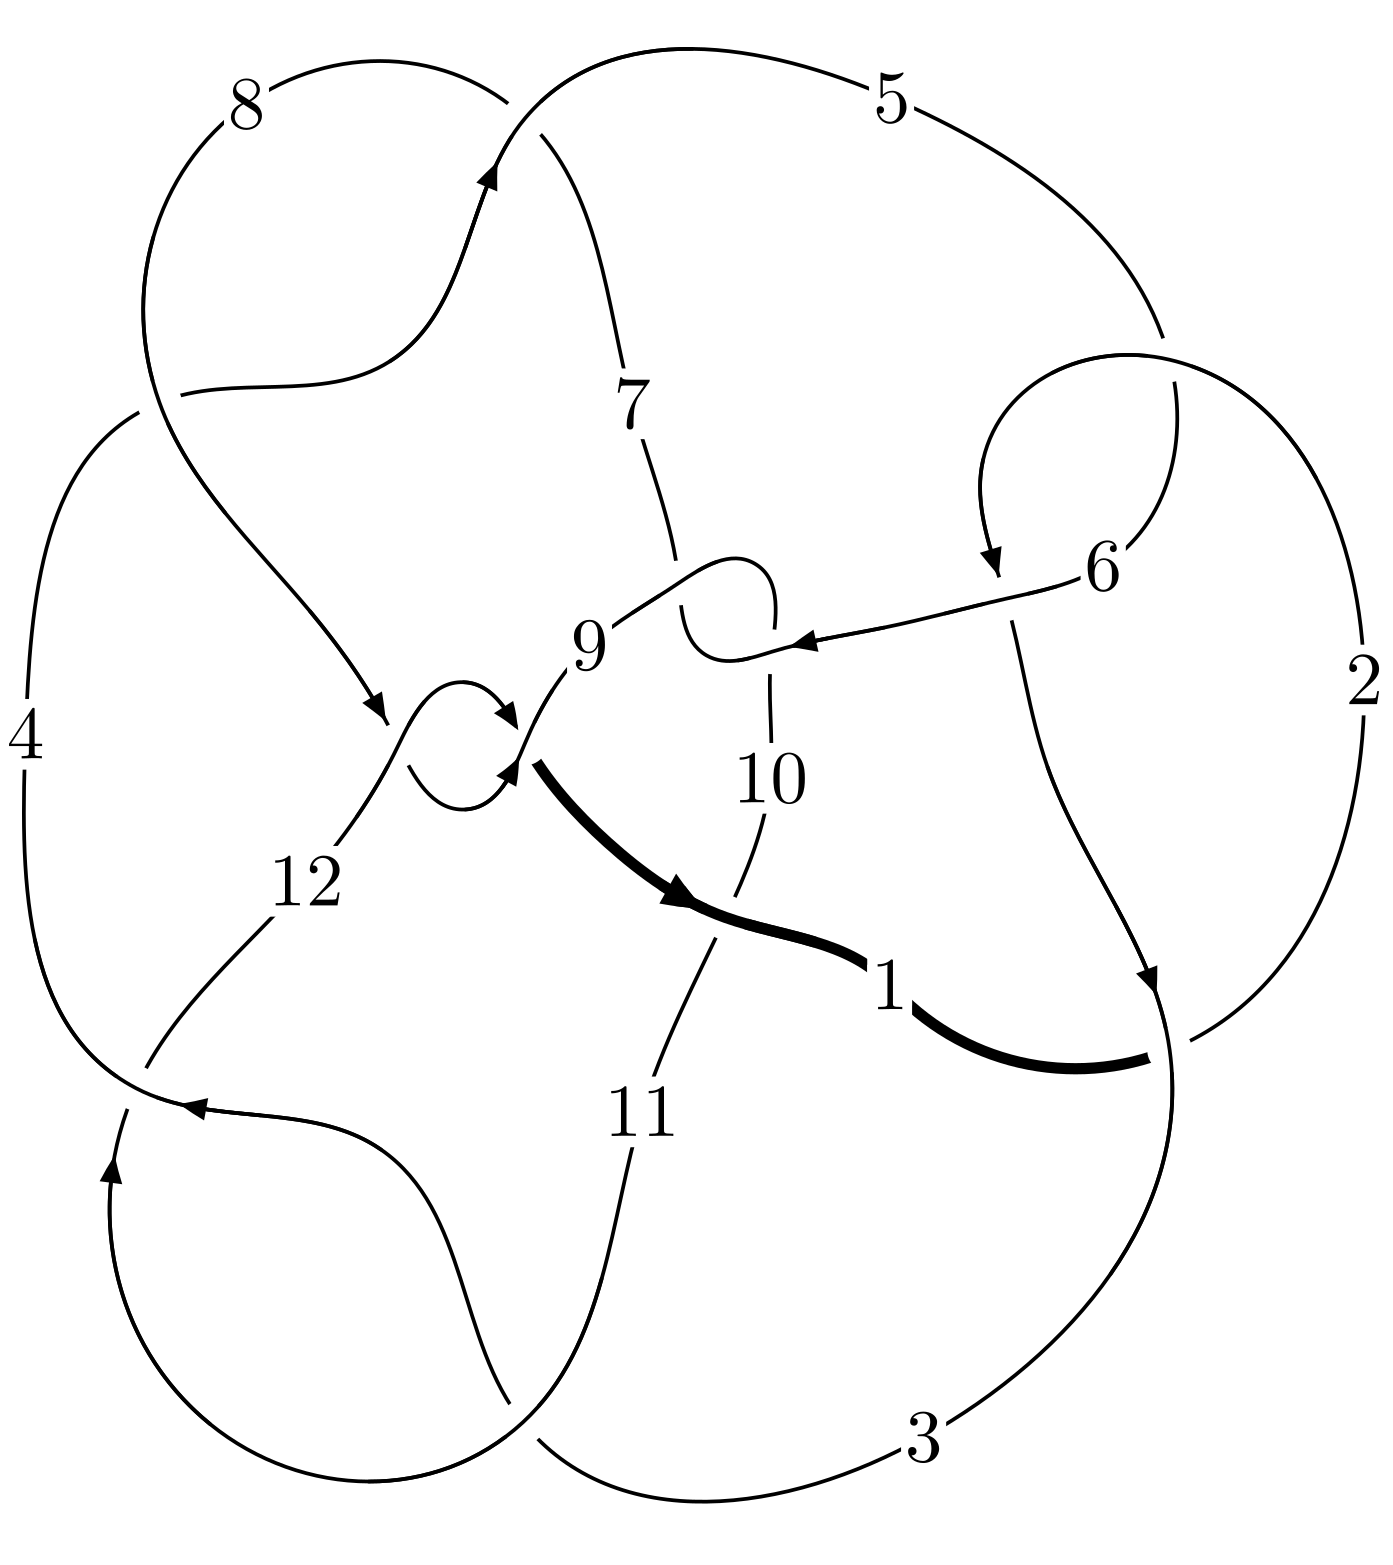
\includegraphics[width=112pt]{../../../GIT/diagram.site/Diagrams/png/2620_12n_0531.png}\\
\ \ \ A knot diagram\footnotemark}&
\allowdisplaybreaks
\textbf{Linearized knot diagam} \\
\cline{2-2}
 &
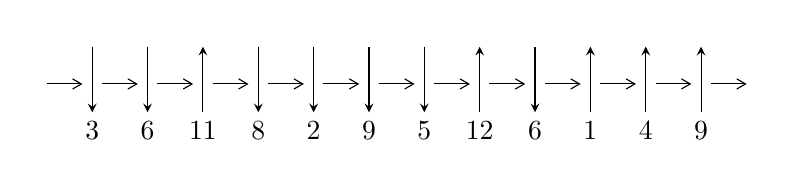
\begin{tikzpicture}[x=20pt, y=17pt]
	% nodes
	\node (C0) at (0, 0) {};
	\node (C1) at (1, 0) {};
	\node (C1U) at (1, +1) {};
	\node (C1D) at (1, -1) {3};

	\node (C2) at (2, 0) {};
	\node (C2U) at (2, +1) {};
	\node (C2D) at (2, -1) {6};

	\node (C3) at (3, 0) {};
	\node (C3U) at (3, +1) {};
	\node (C3D) at (3, -1) {11};

	\node (C4) at (4, 0) {};
	\node (C4U) at (4, +1) {};
	\node (C4D) at (4, -1) {8};

	\node (C5) at (5, 0) {};
	\node (C5U) at (5, +1) {};
	\node (C5D) at (5, -1) {2};

	\node (C6) at (6, 0) {};
	\node (C6U) at (6, +1) {};
	\node (C6D) at (6, -1) {9};

	\node (C7) at (7, 0) {};
	\node (C7U) at (7, +1) {};
	\node (C7D) at (7, -1) {5};

	\node (C8) at (8, 0) {};
	\node (C8U) at (8, +1) {};
	\node (C8D) at (8, -1) {12};

	\node (C9) at (9, 0) {};
	\node (C9U) at (9, +1) {};
	\node (C9D) at (9, -1) {6};

	\node (C10) at (10, 0) {};
	\node (C10U) at (10, +1) {};
	\node (C10D) at (10, -1) {1};

	\node (C11) at (11, 0) {};
	\node (C11U) at (11, +1) {};
	\node (C11D) at (11, -1) {4};

	\node (C12) at (12, 0) {};
	\node (C12U) at (12, +1) {};
	\node (C12D) at (12, -1) {9};
	\node (C13) at (13, 0) {};

	% arrows
	\draw[->,>={angle 60}]
	(C0) edge (C1) (C1) edge (C2) (C2) edge (C3) (C3) edge (C4) (C4) edge (C5) (C5) edge (C6) (C6) edge (C7) (C7) edge (C8) (C8) edge (C9) (C9) edge (C10) (C10) edge (C11) (C11) edge (C12) (C12) edge (C13) ;	\draw[->,>=stealth]
	(C1U) edge (C1D) (C2U) edge (C2D) (C3D) edge (C3U) (C4U) edge (C4D) (C5U) edge (C5D) (C6U) edge (C6D) (C7U) edge (C7D) (C8D) edge (C8U) (C9U) edge (C9D) (C10D) edge (C10U) (C11D) edge (C11U) (C12D) edge (C12U) ;
	\end{tikzpicture} \\
\hhline{~~} \\& 
\textbf{Solving Sequence} \\ \cline{2-2} 
 &
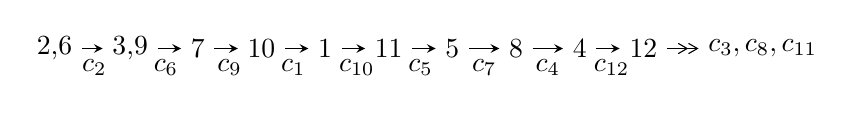
\begin{tikzpicture}[x=23pt, y=7pt]
	% node
	\node (A0) at (-1/8, 0) {2,6};
	\node (A1) at (17/16, 0) {3,9};
	\node (A2) at (17/8, 0) {7};
	\node (A3) at (25/8, 0) {10};
	\node (A4) at (33/8, 0) {1};
	\node (A5) at (41/8, 0) {11};
	\node (A6) at (49/8, 0) {5};
	\node (A7) at (57/8, 0) {8};
	\node (A8) at (65/8, 0) {4};
	\node (A9) at (73/8, 0) {12};
	\node (C1) at (1/2, -1) {$c_{2}$};
	\node (C2) at (13/8, -1) {$c_{6}$};
	\node (C3) at (21/8, -1) {$c_{9}$};
	\node (C4) at (29/8, -1) {$c_{1}$};
	\node (C5) at (37/8, -1) {$c_{10}$};
	\node (C6) at (45/8, -1) {$c_{5}$};
	\node (C7) at (53/8, -1) {$c_{7}$};
	\node (C8) at (61/8, -1) {$c_{4}$};
	\node (C9) at (69/8, -1) {$c_{12}$};
	\node (A10) at (11, 0) {$c_{3},c_{8},c_{11}$};

	% edge
	\draw[->,>=stealth]	
	(A0) edge (A1) (A1) edge (A2) (A2) edge (A3) (A3) edge (A4) (A4) edge (A5) (A5) edge (A6) (A6) edge (A7) (A7) edge (A8) (A8) edge (A9) ;
	\draw[->>,>={angle 60}]	
	(A9) edge (A10);
\end{tikzpicture} \\ 

\end{tabular} \\

\footnotetext{
The image of knot diagram is generated by the software ``\textbf{Draw programme}" developed by Andrew Bartholomew(\url{http://www.layer8.co.uk/maths/draw/index.htm\#Running-draw}), where we modified some parts for our purpose(\url{https://github.com/CATsTAILs/LinksPainter}).
}\phantom \\ \newline 
\centering \textbf{Ideals for irreducible components\footnotemark of $X_{\text{par}}$} 
 
\begin{align*}
I^u_{1}&=\langle 
3.98168\times10^{59} u^{66}-1.61635\times10^{59} u^{65}+\cdots+8.56121\times10^{58} b+6.93366\times10^{59},\\
\phantom{I^u_{1}}&\phantom{= \langle  }-3.91666\times10^{57} u^{66}-2.46674\times10^{59} u^{65}+\cdots+8.56121\times10^{58} a+7.09288\times10^{59},\;u^{67}- u^{66}+\cdots- u-1\rangle \\
I^u_{2}&=\langle 
2 u^{18}-2 u^{17}+\cdots+b-1,\;3 u^{18}- u^{17}+\cdots+a+1,\;u^{19}-5 u^{17}+\cdots+u-1\rangle \\
\\
\end{align*}
\raggedright * 2 irreducible components of $\dim_{\mathbb{C}}=0$, with total 86 representations.\\
\footnotetext{All coefficients of polynomials are rational numbers. But the coefficients are sometimes approximated in decimal forms when there is not enough margin.}
\newpage
\renewcommand{\arraystretch}{1}
\centering \section*{I. $I^u_{1}= \langle 3.98\times10^{59} u^{66}-1.62\times10^{59} u^{65}+\cdots+8.56\times10^{58} b+6.93\times10^{59},\;-3.92\times10^{57} u^{66}-2.47\times10^{59} u^{65}+\cdots+8.56\times10^{58} a+7.09\times10^{59},\;u^{67}- u^{66}+\cdots- u-1 \rangle$}
\flushleft \textbf{(i) Arc colorings}\\
\begin{tabular}{m{7pt} m{180pt} m{7pt} m{180pt} }
\flushright $a_{2}=$&$\begin{pmatrix}1\\0\end{pmatrix}$ \\
\flushright $a_{6}=$&$\begin{pmatrix}0\\u\end{pmatrix}$ \\
\flushright $a_{3}=$&$\begin{pmatrix}1\\u^2\end{pmatrix}$ \\
\flushright $a_{9}=$&$\begin{pmatrix}0.0457489 u^{66}+2.88130 u^{65}+\cdots-27.2442 u-8.28490\\-4.65084 u^{66}+1.88799 u^{65}+\cdots-26.3094 u-8.09892\end{pmatrix}$ \\
\flushright $a_{7}=$&$\begin{pmatrix}-11.1496 u^{66}+2.79842 u^{65}+\cdots-32.9791 u-16.1327\\-5.95825 u^{66}-0.0553272 u^{65}+\cdots-0.0564103 u-4.23853\end{pmatrix}$ \\
\flushright $a_{10}=$&$\begin{pmatrix}0.0457489 u^{66}+2.88130 u^{65}+\cdots-27.2442 u-8.28490\\-0.178100 u^{66}+1.80249 u^{65}+\cdots-23.3366 u-5.17187\end{pmatrix}$ \\
\flushright $a_{1}=$&$\begin{pmatrix}- u^2+1\\- u^4\end{pmatrix}$ \\
\flushright $a_{11}=$&$\begin{pmatrix}-2.13841 u^{66}+4.49817 u^{65}+\cdots-47.2572 u-13.4375\\-3.31213 u^{66}+2.20785 u^{65}+\cdots-30.1781 u-8.48270\end{pmatrix}$ \\
\flushright $a_{5}=$&$\begin{pmatrix}u\\u\end{pmatrix}$ \\
\flushright $a_{8}=$&$\begin{pmatrix}-11.5127 u^{66}+4.27285 u^{65}+\cdots-40.5082 u-18.4704\\-6.32132 u^{66}+1.41910 u^{65}+\cdots-7.58545 u-6.57617\end{pmatrix}$ \\
\flushright $a_{4}=$&$\begin{pmatrix}4.82960 u^{66}-5.95359 u^{65}+\cdots+62.5953 u+18.9033\\6.29424 u^{66}-4.13193 u^{65}+\cdots+48.8147 u+13.7851\end{pmatrix}$ \\
\flushright $a_{12}=$&$\begin{pmatrix}0.918229 u^{66}+1.37577 u^{65}+\cdots-14.7930 u-2.94334\\-0.625938 u^{66}+2.40274 u^{65}+\cdots-25.0155 u-4.68849\end{pmatrix}$\\&\end{tabular}
\flushleft \textbf{(ii) Obstruction class $= -1$}\\~\\
\flushleft \textbf{(iii) Cusp Shapes $= -60.9077 u^{66}+29.1274 u^{65}+\cdots-300.156 u-103.773$}\\~\\
\newpage\renewcommand{\arraystretch}{1}
\flushleft \textbf{(iv) u-Polynomials at the component}\newline \\
\begin{tabular}{m{50pt}|m{274pt}}
Crossings & \hspace{64pt}u-Polynomials at each crossing \\
\hline $$\begin{aligned}c_{1}\end{aligned}$$&$\begin{aligned}
&u^{67}+37 u^{66}+\cdots+7 u+1
\end{aligned}$\\
\hline $$\begin{aligned}c_{2},c_{5}\end{aligned}$$&$\begin{aligned}
&u^{67}+u^{66}+\cdots- u+1
\end{aligned}$\\
\hline $$\begin{aligned}c_{3},c_{11}\end{aligned}$$&$\begin{aligned}
&u^{67}-2 u^{66}+\cdots-89 u+29
\end{aligned}$\\
\hline $$\begin{aligned}c_{4},c_{7}\end{aligned}$$&$\begin{aligned}
&u^{67}-3 u^{66}+\cdots+1479 u+1799
\end{aligned}$\\
\hline $$\begin{aligned}c_{6},c_{9}\end{aligned}$$&$\begin{aligned}
&u^{67}-10 u^{66}+\cdots-14957 u+583
\end{aligned}$\\
\hline $$\begin{aligned}c_{8},c_{12}\end{aligned}$$&$\begin{aligned}
&u^{67}-3 u^{66}+\cdots+1963 u+409
\end{aligned}$\\
\hline $$\begin{aligned}c_{10}\end{aligned}$$&$\begin{aligned}
&u^{67}+6 u^{66}+\cdots+958404 u-46939
\end{aligned}$\\
\hline
\end{tabular}\\~\\
\newpage\renewcommand{\arraystretch}{1}
\flushleft \textbf{(v) Riley Polynomials at the component}\newline \\
\begin{tabular}{m{50pt}|m{274pt}}
Crossings & \hspace{64pt}Riley Polynomials at each crossing \\
\hline $$\begin{aligned}c_{1}\end{aligned}$$&$\begin{aligned}
&y^{67}-5 y^{66}+\cdots+59 y-1
\end{aligned}$\\
\hline $$\begin{aligned}c_{2},c_{5}\end{aligned}$$&$\begin{aligned}
&y^{67}-37 y^{66}+\cdots+7 y-1
\end{aligned}$\\
\hline $$\begin{aligned}c_{3},c_{11}\end{aligned}$$&$\begin{aligned}
&y^{67}-66 y^{66}+\cdots+7283 y-841
\end{aligned}$\\
\hline $$\begin{aligned}c_{4},c_{7}\end{aligned}$$&$\begin{aligned}
&y^{67}+35 y^{66}+\cdots-114931057 y-3236401
\end{aligned}$\\
\hline $$\begin{aligned}c_{6},c_{9}\end{aligned}$$&$\begin{aligned}
&y^{67}-50 y^{66}+\cdots-1103445 y-339889
\end{aligned}$\\
\hline $$\begin{aligned}c_{8},c_{12}\end{aligned}$$&$\begin{aligned}
&y^{67}-43 y^{66}+\cdots+32507091 y-167281
\end{aligned}$\\
\hline $$\begin{aligned}c_{10}\end{aligned}$$&$\begin{aligned}
&y^{67}+22 y^{66}+\cdots+83085423428 y-2203269721
\end{aligned}$\\
\hline
\end{tabular}\\~\\
\newpage\flushleft \textbf{(vi) Complex Volumes and Cusp Shapes}
$$\begin{array}{c|c|c}  
\text{Solutions to }I^u_{1}& \I (\text{vol} + \sqrt{-1}CS) & \text{Cusp shape}\\
 \hline 
\begin{aligned}
u &= \phantom{-}0.252718 + 0.954803 I \\
a &= -0.26765 - 1.61765 I \\
b &= \phantom{-}0.0508940 - 0.0605544 I\end{aligned}
 & \phantom{-}5.44022 + 9.83317 I & \phantom{-}3.49519 - 5.08650 I \\ \hline\begin{aligned}
u &= \phantom{-}0.252718 - 0.954803 I \\
a &= -0.26765 + 1.61765 I \\
b &= \phantom{-}0.0508940 + 0.0605544 I\end{aligned}
 & \phantom{-}5.44022 - 9.83317 I & \phantom{-}3.49519 + 5.08650 I \\ \hline\begin{aligned}
u &= -0.992189 + 0.285907 I \\
a &= \phantom{-}0.299845 - 0.936902 I \\
b &= \phantom{-}0.110971 - 0.511676 I\end{aligned}
 & -0.72386 + 3.39798 I & \phantom{-0.000000 } 0 \\ \hline\begin{aligned}
u &= -0.992189 - 0.285907 I \\
a &= \phantom{-}0.299845 + 0.936902 I \\
b &= \phantom{-}0.110971 + 0.511676 I\end{aligned}
 & -0.72386 - 3.39798 I & \phantom{-0.000000 } 0 \\ \hline\begin{aligned}
u &= \phantom{-}1.003700 + 0.377660 I \\
a &= -0.36326 - 2.02909 I \\
b &= -0.22611 - 1.95101 I\end{aligned}
 & \phantom{-}6.90463 - 5.17042 I & \phantom{-0.000000 } 0 \\ \hline\begin{aligned}
u &= \phantom{-}1.003700 - 0.377660 I \\
a &= -0.36326 + 2.02909 I \\
b &= -0.22611 + 1.95101 I\end{aligned}
 & \phantom{-}6.90463 + 5.17042 I & \phantom{-0.000000 } 0 \\ \hline\begin{aligned}
u &= -0.407354 + 0.830734 I \\
a &= \phantom{-}0.62622 + 1.45214 I \\
b &= \phantom{-}0.0808578 - 0.0470274 I\end{aligned}
 & \phantom{-}1.53350 - 1.63271 I & \phantom{-}4.18307 + 1.16614 I \\ \hline\begin{aligned}
u &= -0.407354 - 0.830734 I \\
a &= \phantom{-}0.62622 - 1.45214 I \\
b &= \phantom{-}0.0808578 + 0.0470274 I\end{aligned}
 & \phantom{-}1.53350 + 1.63271 I & \phantom{-}4.18307 - 1.16614 I \\ \hline\begin{aligned}
u &= -0.999539 + 0.414079 I \\
a &= -0.68465 + 1.36026 I \\
b &= -1.62369 + 0.88630 I\end{aligned}
 & \phantom{-}7.15973 + 0.55296 I & \phantom{-0.000000 } 0 \\ \hline\begin{aligned}
u &= -0.999539 - 0.414079 I \\
a &= -0.68465 - 1.36026 I \\
b &= -1.62369 - 0.88630 I\end{aligned}
 & \phantom{-}7.15973 - 0.55296 I & \phantom{-0.000000 } 0\\
 \hline 
 \end{array}$$\newpage$$\begin{array}{c|c|c}  
\text{Solutions to }I^u_{1}& \I (\text{vol} + \sqrt{-1}CS) & \text{Cusp shape}\\
 \hline 
\begin{aligned}
u &= -0.123677 + 0.896241 I \\
a &= \phantom{-}0.46772 - 1.45771 I \\
b &= \phantom{-}0.188411 + 0.059427 I\end{aligned}
 & -0.54114 - 5.20408 I & \phantom{-}0.74353 + 5.07775 I \\ \hline\begin{aligned}
u &= -0.123677 - 0.896241 I \\
a &= \phantom{-}0.46772 + 1.45771 I \\
b &= \phantom{-}0.188411 - 0.059427 I\end{aligned}
 & -0.54114 + 5.20408 I & \phantom{-}0.74353 - 5.07775 I \\ \hline\begin{aligned}
u &= \phantom{-}0.058282 + 0.894932 I \\
a &= \phantom{-}0.22934 + 1.41748 I \\
b &= -0.420848 + 0.236426 I\end{aligned}
 & \phantom{-}1.96860 + 2.63316 I & \phantom{-}3.47626 - 2.77896 I \\ \hline\begin{aligned}
u &= \phantom{-}0.058282 - 0.894932 I \\
a &= \phantom{-}0.22934 - 1.41748 I \\
b &= -0.420848 - 0.236426 I\end{aligned}
 & \phantom{-}1.96860 - 2.63316 I & \phantom{-}3.47626 + 2.77896 I \\ \hline\begin{aligned}
u &= \phantom{-}0.888129 + 0.007732 I \\
a &= -0.216716 + 0.589577 I \\
b &= \phantom{-}0.397274 - 0.090049 I\end{aligned}
 & -1.42025 + 0.09498 I & -5.88538 + 0.49320 I \\ \hline\begin{aligned}
u &= \phantom{-}0.888129 - 0.007732 I \\
a &= -0.216716 - 0.589577 I \\
b &= \phantom{-}0.397274 + 0.090049 I\end{aligned}
 & -1.42025 - 0.09498 I & -5.88538 - 0.49320 I \\ \hline\begin{aligned}
u &= \phantom{-}0.818749 + 0.312512 I \\
a &= \phantom{-}0.261521 + 0.302439 I \\
b &= -0.94854 - 1.42046 I\end{aligned}
 & \phantom{-}2.49844 - 1.45815 I & \phantom{-}5.05080 + 4.52220 I \\ \hline\begin{aligned}
u &= \phantom{-}0.818749 - 0.312512 I \\
a &= \phantom{-}0.261521 - 0.302439 I \\
b &= -0.94854 + 1.42046 I\end{aligned}
 & \phantom{-}2.49844 + 1.45815 I & \phantom{-}5.05080 - 4.52220 I \\ \hline\begin{aligned}
u &= -0.826794 + 0.261915 I \\
a &= -1.15533 - 0.90370 I \\
b &= -1.65362 + 0.22840 I\end{aligned}
 & \phantom{-}2.29966 + 1.29505 I & \phantom{-}7.24915 - 5.10541 I \\ \hline\begin{aligned}
u &= -0.826794 - 0.261915 I \\
a &= -1.15533 + 0.90370 I \\
b &= -1.65362 - 0.22840 I\end{aligned}
 & \phantom{-}2.29966 - 1.29505 I & \phantom{-}7.24915 + 5.10541 I\\
 \hline 
 \end{array}$$\newpage$$\begin{array}{c|c|c}  
\text{Solutions to }I^u_{1}& \I (\text{vol} + \sqrt{-1}CS) & \text{Cusp shape}\\
 \hline 
\begin{aligned}
u &= -1.062370 + 0.439025 I \\
a &= -0.1189350 + 0.0634968 I \\
b &= \phantom{-}0.08475 - 1.49717 I\end{aligned}
 & \phantom{-}6.23019 + 6.25320 I & \phantom{-0.000000 } 0 \\ \hline\begin{aligned}
u &= -1.062370 - 0.439025 I \\
a &= -0.1189350 - 0.0634968 I \\
b &= \phantom{-}0.08475 + 1.49717 I\end{aligned}
 & \phantom{-}6.23019 - 6.25320 I & \phantom{-0.000000 } 0 \\ \hline\begin{aligned}
u &= \phantom{-}1.078930 + 0.400055 I \\
a &= \phantom{-}0.966889 - 0.461546 I \\
b &= \phantom{-}1.50362 + 0.72539 I\end{aligned}
 & \phantom{-}5.90798 - 0.58176 I & \phantom{-0.000000 } 0 \\ \hline\begin{aligned}
u &= \phantom{-}1.078930 - 0.400055 I \\
a &= \phantom{-}0.966889 + 0.461546 I \\
b &= \phantom{-}1.50362 - 0.72539 I\end{aligned}
 & \phantom{-}5.90798 + 0.58176 I & \phantom{-0.000000 } 0 \\ \hline\begin{aligned}
u &= \phantom{-}1.139110 + 0.269989 I \\
a &= -1.336930 - 0.044286 I \\
b &= -2.77376 + 0.09507 I\end{aligned}
 & -3.24471 - 0.99304 I & \phantom{-0.000000 } 0 \\ \hline\begin{aligned}
u &= \phantom{-}1.139110 - 0.269989 I \\
a &= -1.336930 + 0.044286 I \\
b &= -2.77376 - 0.09507 I\end{aligned}
 & -3.24471 + 0.99304 I & \phantom{-0.000000 } 0 \\ \hline\begin{aligned}
u &= -0.870317 + 0.790370 I \\
a &= -0.382693 - 0.266135 I \\
b &= -0.207034 - 0.348229 I\end{aligned}
 & \phantom{-}4.48838 + 2.95750 I & \phantom{-0.000000 } 0 \\ \hline\begin{aligned}
u &= -0.870317 - 0.790370 I \\
a &= -0.382693 + 0.266135 I \\
b &= -0.207034 + 0.348229 I\end{aligned}
 & \phantom{-}4.48838 - 2.95750 I & \phantom{-0.000000 } 0 \\ \hline\begin{aligned}
u &= \phantom{-}0.790678 + 0.880867 I \\
a &= \phantom{-}0.506555 - 0.282964 I \\
b &= -0.109676 + 0.105383 I\end{aligned}
 & \phantom{-}9.15754 - 5.60614 I & \phantom{-0.000000 } 0 \\ \hline\begin{aligned}
u &= \phantom{-}0.790678 - 0.880867 I \\
a &= \phantom{-}0.506555 + 0.282964 I \\
b &= -0.109676 - 0.105383 I\end{aligned}
 & \phantom{-}9.15754 + 5.60614 I & \phantom{-0.000000 } 0\\
 \hline 
 \end{array}$$\newpage$$\begin{array}{c|c|c}  
\text{Solutions to }I^u_{1}& \I (\text{vol} + \sqrt{-1}CS) & \text{Cusp shape}\\
 \hline 
\begin{aligned}
u &= \phantom{-}0.126398 + 0.792019 I \\
a &= -0.34046 + 1.55116 I \\
b &= \phantom{-}0.141669 + 0.103536 I\end{aligned}
 & -2.45188 - 0.35885 I & -3.63602 + 0.23516 I \\ \hline\begin{aligned}
u &= \phantom{-}0.126398 - 0.792019 I \\
a &= -0.34046 - 1.55116 I \\
b &= \phantom{-}0.141669 - 0.103536 I\end{aligned}
 & -2.45188 + 0.35885 I & -3.63602 - 0.23516 I \\ \hline\begin{aligned}
u &= \phantom{-}0.962593 + 0.817723 I \\
a &= \phantom{-}0.208169 - 0.306861 I \\
b &= \phantom{-}0.616506 - 0.727645 I\end{aligned}
 & \phantom{-}8.63874 - 0.64633 I & \phantom{-0.000000 } 0 \\ \hline\begin{aligned}
u &= \phantom{-}0.962593 - 0.817723 I \\
a &= \phantom{-}0.208169 + 0.306861 I \\
b &= \phantom{-}0.616506 + 0.727645 I\end{aligned}
 & \phantom{-}8.63874 + 0.64633 I & \phantom{-0.000000 } 0 \\ \hline\begin{aligned}
u &= \phantom{-}1.196810 + 0.425223 I \\
a &= \phantom{-}0.992583 + 0.428060 I \\
b &= \phantom{-}2.34581 + 0.17564 I\end{aligned}
 & -2.51573 - 3.88919 I & \phantom{-0.000000 } 0 \\ \hline\begin{aligned}
u &= \phantom{-}1.196810 - 0.425223 I \\
a &= \phantom{-}0.992583 - 0.428060 I \\
b &= \phantom{-}2.34581 - 0.17564 I\end{aligned}
 & -2.51573 + 3.88919 I & \phantom{-0.000000 } 0 \\ \hline\begin{aligned}
u &= -0.095962 + 0.718089 I \\
a &= -0.870727 - 1.075470 I \\
b &= -0.514432 + 0.209197 I\end{aligned}
 & \phantom{-}1.107230 - 0.185144 I & \phantom{-}4.79017 - 0.71844 I \\ \hline\begin{aligned}
u &= -0.095962 - 0.718089 I \\
a &= -0.870727 + 1.075470 I \\
b &= -0.514432 - 0.209197 I\end{aligned}
 & \phantom{-}1.107230 + 0.185144 I & \phantom{-}4.79017 + 0.71844 I \\ \hline\begin{aligned}
u &= -1.222550 + 0.406422 I \\
a &= \phantom{-}1.373620 + 0.083582 I \\
b &= \phantom{-}2.55563 + 0.01499 I\end{aligned}
 & -6.39757 + 4.49155 I & \phantom{-0.000000 } 0 \\ \hline\begin{aligned}
u &= -1.222550 - 0.406422 I \\
a &= \phantom{-}1.373620 - 0.083582 I \\
b &= \phantom{-}2.55563 - 0.01499 I\end{aligned}
 & -6.39757 - 4.49155 I & \phantom{-0.000000 } 0\\
 \hline 
 \end{array}$$\newpage$$\begin{array}{c|c|c}  
\text{Solutions to }I^u_{1}& \I (\text{vol} + \sqrt{-1}CS) & \text{Cusp shape}\\
 \hline 
\begin{aligned}
u &= -1.190060 + 0.501845 I \\
a &= -0.803790 - 0.598061 I \\
b &= -1.74421 - 0.52832 I\end{aligned}
 & -1.97091 + 4.80612 I & \phantom{-0.000000 } 0 \\ \hline\begin{aligned}
u &= -1.190060 - 0.501845 I \\
a &= -0.803790 + 0.598061 I \\
b &= -1.74421 + 0.52832 I\end{aligned}
 & -1.97091 - 4.80612 I & \phantom{-0.000000 } 0 \\ \hline\begin{aligned}
u &= -1.150470 + 0.612288 I \\
a &= \phantom{-}1.177240 + 0.454917 I \\
b &= \phantom{-}2.37784 + 0.80163 I\end{aligned}
 & -0.72397 + 7.05260 I & \phantom{-0.000000 } 0 \\ \hline\begin{aligned}
u &= -1.150470 - 0.612288 I \\
a &= \phantom{-}1.177240 - 0.454917 I \\
b &= \phantom{-}2.37784 - 0.80163 I\end{aligned}
 & -0.72397 - 7.05260 I & \phantom{-0.000000 } 0 \\ \hline\begin{aligned}
u &= \phantom{-}1.205080 + 0.518507 I \\
a &= -1.148840 + 0.185650 I \\
b &= -2.18745 + 0.58972 I\end{aligned}
 & -5.59025 - 4.50406 I & \phantom{-0.000000 } 0 \\ \hline\begin{aligned}
u &= \phantom{-}1.205080 - 0.518507 I \\
a &= -1.148840 - 0.185650 I \\
b &= -2.18745 - 0.58972 I\end{aligned}
 & -5.59025 + 4.50406 I & \phantom{-0.000000 } 0 \\ \hline\begin{aligned}
u &= \phantom{-}1.264300 + 0.382115 I \\
a &= \phantom{-}1.009520 - 0.475156 I \\
b &= \phantom{-}2.03470 - 0.67673 I\end{aligned}
 & -4.90333 + 0.82967 I & \phantom{-0.000000 } 0 \\ \hline\begin{aligned}
u &= \phantom{-}1.264300 - 0.382115 I \\
a &= \phantom{-}1.009520 + 0.475156 I \\
b &= \phantom{-}2.03470 + 0.67673 I\end{aligned}
 & -4.90333 - 0.82967 I & \phantom{-0.000000 } 0 \\ \hline\begin{aligned}
u &= -1.265610 + 0.421354 I \\
a &= \phantom{-}0.943794 - 0.070930 I \\
b &= \phantom{-}1.70252 + 0.53403 I\end{aligned}
 & -2.14236 + 1.98560 I & \phantom{-0.000000 } 0 \\ \hline\begin{aligned}
u &= -1.265610 - 0.421354 I \\
a &= \phantom{-}0.943794 + 0.070930 I \\
b &= \phantom{-}1.70252 - 0.53403 I\end{aligned}
 & -2.14236 - 1.98560 I & \phantom{-0.000000 } 0\\
 \hline 
 \end{array}$$\newpage$$\begin{array}{c|c|c}  
\text{Solutions to }I^u_{1}& \I (\text{vol} + \sqrt{-1}CS) & \text{Cusp shape}\\
 \hline 
\begin{aligned}
u &= -1.308880 + 0.267985 I \\
a &= -1.123170 - 0.336397 I \\
b &= -2.17522 - 0.78717 I\end{aligned}
 & \phantom{-}0.18085 - 5.77518 I & \phantom{-0.000000 } 0 \\ \hline\begin{aligned}
u &= -1.308880 - 0.267985 I \\
a &= -1.123170 + 0.336397 I \\
b &= -2.17522 + 0.78717 I\end{aligned}
 & \phantom{-}0.18085 + 5.77518 I & \phantom{-0.000000 } 0 \\ \hline\begin{aligned}
u &= \phantom{-}1.245830 + 0.493179 I \\
a &= -1.43974 + 0.17283 I \\
b &= -2.43608 - 0.13299 I\end{aligned}
 & -1.63829 - 7.60166 I & \phantom{-0.000000 } 0 \\ \hline\begin{aligned}
u &= \phantom{-}1.245830 - 0.493179 I \\
a &= -1.43974 - 0.17283 I \\
b &= -2.43608 + 0.13299 I\end{aligned}
 & -1.63829 + 7.60166 I & \phantom{-0.000000 } 0 \\ \hline\begin{aligned}
u &= -1.235560 + 0.521982 I \\
a &= -1.234460 + 0.179282 I \\
b &= -2.59326 + 0.12435 I\end{aligned}
 & -3.91456 + 10.33250 I & \phantom{-0.000000 } 0 \\ \hline\begin{aligned}
u &= -1.235560 - 0.521982 I \\
a &= -1.234460 - 0.179282 I \\
b &= -2.59326 - 0.12435 I\end{aligned}
 & -3.91456 - 10.33250 I & \phantom{-0.000000 } 0 \\ \hline\begin{aligned}
u &= \phantom{-}1.225640 + 0.591919 I \\
a &= \phantom{-}1.41828 + 0.02698 I \\
b &= \phantom{-}2.74705 + 0.09456 I\end{aligned}
 & \phantom{-}2.4570 - 15.4421 I & \phantom{-0.000000 } 0 \\ \hline\begin{aligned}
u &= \phantom{-}1.225640 - 0.591919 I \\
a &= \phantom{-}1.41828 - 0.02698 I \\
b &= \phantom{-}2.74705 - 0.09456 I\end{aligned}
 & \phantom{-}2.4570 + 15.4421 I & \phantom{-0.000000 } 0 \\ \hline\begin{aligned}
u &= \phantom{-}0.596336 + 0.122603 I \\
a &= \phantom{-}2.26885 + 1.87775 I \\
b &= \phantom{-}2.01780 + 0.76808 I\end{aligned}
 & \phantom{-}8.49281 + 2.29820 I & \phantom{-}6.25286 - 4.10564 I \\ \hline\begin{aligned}
u &= \phantom{-}0.596336 - 0.122603 I \\
a &= \phantom{-}2.26885 - 1.87775 I \\
b &= \phantom{-}2.01780 - 0.76808 I\end{aligned}
 & \phantom{-}8.49281 - 2.29820 I & \phantom{-}6.25286 + 4.10564 I\\
 \hline 
 \end{array}$$\newpage$$\begin{array}{c|c|c}  
\text{Solutions to }I^u_{1}& \I (\text{vol} + \sqrt{-1}CS) & \text{Cusp shape}\\
 \hline 
\begin{aligned}
u &= \phantom{-}0.592523\phantom{ +0.000000I} \\
a &= -0.956423\phantom{ +0.000000I} \\
b &= \phantom{-}0.295328\phantom{ +0.000000I}\end{aligned}
 & -1.13446\phantom{ +0.000000I} & -10.7330\phantom{ +0.000000I} \\ \hline\begin{aligned}
u &= -0.497958 + 0.215908 I \\
a &= \phantom{-}0.68502 - 2.08646 I \\
b &= \phantom{-}1.76295 - 0.08326 I\end{aligned}
 & \phantom{-}8.74993 + 2.73352 I & \phantom{-}4.86441 - 2.29828 I \\ \hline\begin{aligned}
u &= -0.497958 - 0.215908 I \\
a &= \phantom{-}0.68502 + 2.08646 I \\
b &= \phantom{-}1.76295 + 0.08326 I\end{aligned}
 & \phantom{-}8.74993 - 2.73352 I & \phantom{-}4.86441 + 2.29828 I \\ \hline\begin{aligned}
u &= -0.291880 + 0.442830 I \\
a &= -0.880180 - 0.165991 I \\
b &= -0.525541 + 0.323507 I\end{aligned}
 & \phantom{-}1.258410 - 0.412792 I & \phantom{-}6.74896 + 1.13109 I \\ \hline\begin{aligned}
u &= -0.291880 - 0.442830 I \\
a &= -0.880180 + 0.165991 I \\
b &= -0.525541 - 0.323507 I\end{aligned}
 & \phantom{-}1.258410 + 0.412792 I & \phantom{-}6.74896 - 1.13109 I \\ \hline\begin{aligned}
u &= -0.108371 + 0.359754 I \\
a &= -2.08944 - 0.74875 I \\
b &= \phantom{-}1.272570 - 0.328628 I\end{aligned}
 & \phantom{-}8.55502 - 2.64869 I & \phantom{-}5.98628 + 2.06746 I \\ \hline\begin{aligned}
u &= -0.108371 - 0.359754 I \\
a &= -2.08944 + 0.74875 I \\
b &= \phantom{-}1.272570 + 0.328628 I\end{aligned}
 & \phantom{-}8.55502 + 2.64869 I & \phantom{-}5.98628 - 2.06746 I\\
 \hline 
 \end{array}$$\newpage\newpage\renewcommand{\arraystretch}{1}
\centering \section*{II. $I^u_{2}= \langle 2 u^{18}-2 u^{17}+\cdots+b-1,\;3 u^{18}- u^{17}+\cdots+a+1,\;u^{19}-5 u^{17}+\cdots+u-1 \rangle$}
\flushleft \textbf{(i) Arc colorings}\\
\begin{tabular}{m{7pt} m{180pt} m{7pt} m{180pt} }
\flushright $a_{2}=$&$\begin{pmatrix}1\\0\end{pmatrix}$ \\
\flushright $a_{6}=$&$\begin{pmatrix}0\\u\end{pmatrix}$ \\
\flushright $a_{3}=$&$\begin{pmatrix}1\\u^2\end{pmatrix}$ \\
\flushright $a_{9}=$&$\begin{pmatrix}-3 u^{18}+u^{17}+\cdots-4 u-1\\-2 u^{18}+2 u^{17}+\cdots-5 u^2+1\end{pmatrix}$ \\
\flushright $a_{7}=$&$\begin{pmatrix}3 u^{18}-3 u^{17}+\cdots+4 u-4\\5 u^{18}-3 u^{17}+\cdots+10 u-3\end{pmatrix}$ \\
\flushright $a_{10}=$&$\begin{pmatrix}-3 u^{18}+u^{17}+\cdots-4 u-1\\-4 u^{18}+3 u^{17}+\cdots-4 u+2\end{pmatrix}$ \\
\flushright $a_{1}=$&$\begin{pmatrix}- u^2+1\\- u^4\end{pmatrix}$ \\
\flushright $a_{11}=$&$\begin{pmatrix}-3 u^{18}+u^{17}+\cdots- u-2\\-3 u^{18}+3 u^{17}+\cdots- u+1\end{pmatrix}$ \\
\flushright $a_{5}=$&$\begin{pmatrix}u\\u\end{pmatrix}$ \\
\flushright $a_{8}=$&$\begin{pmatrix}3 u^{18}-3 u^{17}+\cdots+2 u-4\\5 u^{18}-3 u^{17}+\cdots+8 u-3\end{pmatrix}$ \\
\flushright $a_{4}=$&$\begin{pmatrix}u^{18}-6 u^{16}+\cdots-2 u^2+8 u\\-2 u^{18}+u^{17}+\cdots+2 u-1\end{pmatrix}$ \\
\flushright $a_{12}=$&$\begin{pmatrix}2 u^{18}-4 u^{17}+\cdots+3 u-3\\3 u^{18}-4 u^{17}+\cdots+4 u-3\end{pmatrix}$\\&\end{tabular}
\flushleft \textbf{(ii) Obstruction class $= 1$}\\~\\
\flushleft \textbf{(iii) Cusp Shapes $= 7 u^{18}+3 u^{17}-33 u^{16}-14 u^{15}+87 u^{14}+36 u^{13}-144 u^{12}-65 u^{11}+165 u^{10}+92 u^9-115 u^8-96 u^7+35 u^6+79 u^5+21 u^4-48 u^3-25 u^2+11 u+8$}\\~\\
\newpage\renewcommand{\arraystretch}{1}
\flushleft \textbf{(iv) u-Polynomials at the component}\newline \\
\begin{tabular}{m{50pt}|m{274pt}}
Crossings & \hspace{64pt}u-Polynomials at each crossing \\
\hline $$\begin{aligned}c_{1}\end{aligned}$$&$\begin{aligned}
&u^{19}-10 u^{18}+\cdots+11 u-1
\end{aligned}$\\
\hline $$\begin{aligned}c_{2}\end{aligned}$$&$\begin{aligned}
&u^{19}-5 u^{17}+\cdots+u-1
\end{aligned}$\\
\hline $$\begin{aligned}c_{3}\end{aligned}$$&$\begin{aligned}
&u^{19}+u^{18}+\cdots+u-1
\end{aligned}$\\
\hline $$\begin{aligned}c_{4}\end{aligned}$$&$\begin{aligned}
&u^{19}-2 u^{18}+\cdots- u-1
\end{aligned}$\\
\hline $$\begin{aligned}c_{5}\end{aligned}$$&$\begin{aligned}
&u^{19}-5 u^{17}+\cdots+u+1
\end{aligned}$\\
\hline $$\begin{aligned}c_{6}\end{aligned}$$&$\begin{aligned}
&u^{19}-3 u^{18}+\cdots-7 u-1
\end{aligned}$\\
\hline $$\begin{aligned}c_{7}\end{aligned}$$&$\begin{aligned}
&u^{19}+2 u^{18}+\cdots- u+1
\end{aligned}$\\
\hline $$\begin{aligned}c_{8}\end{aligned}$$&$\begin{aligned}
&u^{19}-4 u^{18}+\cdots+u+1
\end{aligned}$\\
\hline $$\begin{aligned}c_{9}\end{aligned}$$&$\begin{aligned}
&u^{19}+3 u^{18}+\cdots-7 u+1
\end{aligned}$\\
\hline $$\begin{aligned}c_{10}\end{aligned}$$&$\begin{aligned}
&u^{19}- u^{18}+\cdots+236 u+43
\end{aligned}$\\
\hline $$\begin{aligned}c_{11}\end{aligned}$$&$\begin{aligned}
&u^{19}- u^{18}+\cdots+u+1
\end{aligned}$\\
\hline $$\begin{aligned}c_{12}\end{aligned}$$&$\begin{aligned}
&u^{19}+4 u^{18}+\cdots+u-1
\end{aligned}$\\
\hline
\end{tabular}\\~\\
\newpage\renewcommand{\arraystretch}{1}
\flushleft \textbf{(v) Riley Polynomials at the component}\newline \\
\begin{tabular}{m{50pt}|m{274pt}}
Crossings & \hspace{64pt}Riley Polynomials at each crossing \\
\hline $$\begin{aligned}c_{1}\end{aligned}$$&$\begin{aligned}
&y^{19}+6 y^{18}+\cdots+27 y-1
\end{aligned}$\\
\hline $$\begin{aligned}c_{2},c_{5}\end{aligned}$$&$\begin{aligned}
&y^{19}-10 y^{18}+\cdots+11 y-1
\end{aligned}$\\
\hline $$\begin{aligned}c_{3},c_{11}\end{aligned}$$&$\begin{aligned}
&y^{19}-23 y^{18}+\cdots-13 y-1
\end{aligned}$\\
\hline $$\begin{aligned}c_{4},c_{7}\end{aligned}$$&$\begin{aligned}
&y^{19}+10 y^{18}+\cdots+3 y-1
\end{aligned}$\\
\hline $$\begin{aligned}c_{6},c_{9}\end{aligned}$$&$\begin{aligned}
&y^{19}-3 y^{18}+\cdots+35 y-1
\end{aligned}$\\
\hline $$\begin{aligned}c_{8},c_{12}\end{aligned}$$&$\begin{aligned}
&y^{19}-16 y^{18}+\cdots-5 y-1
\end{aligned}$\\
\hline $$\begin{aligned}c_{10}\end{aligned}$$&$\begin{aligned}
&y^{19}-3 y^{18}+\cdots+26284 y-1849
\end{aligned}$\\
\hline
\end{tabular}\\~\\
\newpage\flushleft \textbf{(vi) Complex Volumes and Cusp Shapes}
$$\begin{array}{c|c|c}  
\text{Solutions to }I^u_{2}& \I (\text{vol} + \sqrt{-1}CS) & \text{Cusp shape}\\
 \hline 
\begin{aligned}
u &= -0.978751 + 0.307404 I \\
a &= -0.08895 - 1.68231 I \\
b &= \phantom{-}0.094662 - 0.624680 I\end{aligned}
 & \phantom{-}7.28503 + 4.10785 I & \phantom{-}2.95414 - 2.86490 I \\ \hline\begin{aligned}
u &= -0.978751 - 0.307404 I \\
a &= -0.08895 + 1.68231 I \\
b &= \phantom{-}0.094662 + 0.624680 I\end{aligned}
 & \phantom{-}7.28503 - 4.10785 I & \phantom{-}2.95414 + 2.86490 I \\ \hline\begin{aligned}
u &= \phantom{-}0.904209 + 0.228834 I \\
a &= \phantom{-}0.786990 - 0.518544 I \\
b &= \phantom{-}1.44158 + 0.87989 I\end{aligned}
 & \phantom{-}1.67334 - 1.02006 I & -5.81141 - 0.72669 I \\ \hline\begin{aligned}
u &= \phantom{-}0.904209 - 0.228834 I \\
a &= \phantom{-}0.786990 + 0.518544 I \\
b &= \phantom{-}1.44158 - 0.87989 I\end{aligned}
 & \phantom{-}1.67334 + 1.02006 I & -5.81141 + 0.72669 I \\ \hline\begin{aligned}
u &= \phantom{-}0.818844 + 0.700124 I \\
a &= -0.333710 - 0.781860 I \\
b &= -0.51330 - 1.32368 I\end{aligned}
 & \phantom{-}10.34880 - 4.45139 I & \phantom{-}6.18516 + 3.57443 I \\ \hline\begin{aligned}
u &= \phantom{-}0.818844 - 0.700124 I \\
a &= -0.333710 + 0.781860 I \\
b &= -0.51330 + 1.32368 I\end{aligned}
 & \phantom{-}10.34880 + 4.45139 I & \phantom{-}6.18516 - 3.57443 I \\ \hline\begin{aligned}
u &= -0.880057 + 0.723725 I \\
a &= -0.183448 - 0.085198 I \\
b &= \phantom{-}0.138934 - 0.604807 I\end{aligned}
 & \phantom{-}4.90128 + 2.76357 I & \phantom{-}8.38876 + 0.35727 I \\ \hline\begin{aligned}
u &= -0.880057 - 0.723725 I \\
a &= -0.183448 + 0.085198 I \\
b &= \phantom{-}0.138934 + 0.604807 I\end{aligned}
 & \phantom{-}4.90128 - 2.76357 I & \phantom{-}8.38876 - 0.35727 I \\ \hline\begin{aligned}
u &= -0.787321 + 0.274997 I \\
a &= -1.42135 + 0.91420 I \\
b &= -2.37267 + 1.42356 I\end{aligned}
 & \phantom{-}8.01888 - 1.56355 I & \phantom{-}1.27949 - 2.89433 I \\ \hline\begin{aligned}
u &= -0.787321 - 0.274997 I \\
a &= -1.42135 - 0.91420 I \\
b &= -2.37267 - 1.42356 I\end{aligned}
 & \phantom{-}8.01888 + 1.56355 I & \phantom{-}1.27949 + 2.89433 I\\
 \hline 
 \end{array}$$\newpage$$\begin{array}{c|c|c}  
\text{Solutions to }I^u_{2}& \I (\text{vol} + \sqrt{-1}CS) & \text{Cusp shape}\\
 \hline 
\begin{aligned}
u &= \phantom{-}0.940062 + 0.692222 I \\
a &= \phantom{-}0.550056 + 0.651231 I \\
b &= \phantom{-}0.133210 + 0.249610 I\end{aligned}
 & \phantom{-}9.96906 - 0.91166 I & \phantom{-}6.80985 + 1.74521 I \\ \hline\begin{aligned}
u &= \phantom{-}0.940062 - 0.692222 I \\
a &= \phantom{-}0.550056 - 0.651231 I \\
b &= \phantom{-}0.133210 - 0.249610 I\end{aligned}
 & \phantom{-}9.96906 + 0.91166 I & \phantom{-}6.80985 - 1.74521 I \\ \hline\begin{aligned}
u &= -0.233447 + 0.755562 I \\
a &= \phantom{-}0.49290 + 1.41879 I \\
b &= \phantom{-}0.316972 - 0.038293 I\end{aligned}
 & -0.214249 - 0.827859 I & -0.372742 + 0.698304 I \\ \hline\begin{aligned}
u &= -0.233447 - 0.755562 I \\
a &= \phantom{-}0.49290 - 1.41879 I \\
b &= \phantom{-}0.316972 + 0.038293 I\end{aligned}
 & -0.214249 + 0.827859 I & -0.372742 - 0.698304 I \\ \hline\begin{aligned}
u &= \phantom{-}1.193260 + 0.407397 I \\
a &= -1.117000 - 0.146511 I \\
b &= -2.25532 + 0.23263 I\end{aligned}
 & -4.05195 - 2.93073 I & -3.39124 + 2.59909 I \\ \hline\begin{aligned}
u &= \phantom{-}1.193260 - 0.407397 I \\
a &= -1.117000 + 0.146511 I \\
b &= -2.25532 - 0.23263 I\end{aligned}
 & -4.05195 + 2.93073 I & -3.39124 - 2.59909 I \\ \hline\begin{aligned}
u &= -1.199490 + 0.536666 I \\
a &= \phantom{-}1.122270 + 0.371800 I \\
b &= \phantom{-}2.14595 + 0.39527 I\end{aligned}
 & -3.09315 + 5.79872 I & -2.42694 - 4.74421 I \\ \hline\begin{aligned}
u &= -1.199490 - 0.536666 I \\
a &= \phantom{-}1.122270 - 0.371800 I \\
b &= \phantom{-}2.14595 - 0.39527 I\end{aligned}
 & -3.09315 - 5.79872 I & -2.42694 + 4.74421 I \\ \hline\begin{aligned}
u &= \phantom{-}0.445385\phantom{ +0.000000I} \\
a &= -1.61551\phantom{ +0.000000I} \\
b &= \phantom{-}0.739953\phantom{ +0.000000I}\end{aligned}
 & -0.586933\phantom{ +0.000000I} & \phantom{-}5.76990\phantom{ +0.000000I}\\
 \hline 
 \end{array}$$\newpage
\newpage\renewcommand{\arraystretch}{1}
\centering \section*{ III. u-Polynomials}
\begin{tabular}{m{50pt}|m{274pt}}
Crossings & \hspace{64pt}u-Polynomials at each crossing \\
\hline $$\begin{aligned}c_{1}\end{aligned}$$&$\begin{aligned}
&(u^{19}-10 u^{18}+\cdots+11 u-1)(u^{67}+37 u^{66}+\cdots+7 u+1)
\end{aligned}$\\
\hline $$\begin{aligned}c_{2}\end{aligned}$$&$\begin{aligned}
&(u^{19}-5 u^{17}+\cdots+u-1)(u^{67}+u^{66}+\cdots- u+1)
\end{aligned}$\\
\hline $$\begin{aligned}c_{3}\end{aligned}$$&$\begin{aligned}
&(u^{19}+u^{18}+\cdots+u-1)(u^{67}-2 u^{66}+\cdots-89 u+29)
\end{aligned}$\\
\hline $$\begin{aligned}c_{4}\end{aligned}$$&$\begin{aligned}
&(u^{19}-2 u^{18}+\cdots- u-1)(u^{67}-3 u^{66}+\cdots+1479 u+1799)
\end{aligned}$\\
\hline $$\begin{aligned}c_{5}\end{aligned}$$&$\begin{aligned}
&(u^{19}-5 u^{17}+\cdots+u+1)(u^{67}+u^{66}+\cdots- u+1)
\end{aligned}$\\
\hline $$\begin{aligned}c_{6}\end{aligned}$$&$\begin{aligned}
&(u^{19}-3 u^{18}+\cdots-7 u-1)(u^{67}-10 u^{66}+\cdots-14957 u+583)
\end{aligned}$\\
\hline $$\begin{aligned}c_{7}\end{aligned}$$&$\begin{aligned}
&(u^{19}+2 u^{18}+\cdots- u+1)(u^{67}-3 u^{66}+\cdots+1479 u+1799)
\end{aligned}$\\
\hline $$\begin{aligned}c_{8}\end{aligned}$$&$\begin{aligned}
&(u^{19}-4 u^{18}+\cdots+u+1)(u^{67}-3 u^{66}+\cdots+1963 u+409)
\end{aligned}$\\
\hline $$\begin{aligned}c_{9}\end{aligned}$$&$\begin{aligned}
&(u^{19}+3 u^{18}+\cdots-7 u+1)(u^{67}-10 u^{66}+\cdots-14957 u+583)
\end{aligned}$\\
\hline $$\begin{aligned}c_{10}\end{aligned}$$&$\begin{aligned}
&(u^{19}- u^{18}+\cdots+236 u+43)(u^{67}+6 u^{66}+\cdots+958404 u-46939)
\end{aligned}$\\
\hline $$\begin{aligned}c_{11}\end{aligned}$$&$\begin{aligned}
&(u^{19}- u^{18}+\cdots+u+1)(u^{67}-2 u^{66}+\cdots-89 u+29)
\end{aligned}$\\
\hline $$\begin{aligned}c_{12}\end{aligned}$$&$\begin{aligned}
&(u^{19}+4 u^{18}+\cdots+u-1)(u^{67}-3 u^{66}+\cdots+1963 u+409)
\end{aligned}$\\
\hline
\end{tabular}\newpage\renewcommand{\arraystretch}{1}
\centering \section*{ IV. Riley Polynomials}
\begin{tabular}{m{50pt}|m{274pt}}
Crossings & \hspace{64pt}Riley Polynomials at each crossing \\
\hline $$\begin{aligned}c_{1}\end{aligned}$$&$\begin{aligned}
&(y^{19}+6 y^{18}+\cdots+27 y-1)(y^{67}-5 y^{66}+\cdots+59 y-1)
\end{aligned}$\\
\hline $$\begin{aligned}c_{2},c_{5}\end{aligned}$$&$\begin{aligned}
&(y^{19}-10 y^{18}+\cdots+11 y-1)(y^{67}-37 y^{66}+\cdots+7 y-1)
\end{aligned}$\\
\hline $$\begin{aligned}c_{3},c_{11}\end{aligned}$$&$\begin{aligned}
&(y^{19}-23 y^{18}+\cdots-13 y-1)(y^{67}-66 y^{66}+\cdots+7283 y-841)
\end{aligned}$\\
\hline $$\begin{aligned}c_{4},c_{7}\end{aligned}$$&$\begin{aligned}
&(y^{19}+10 y^{18}+\cdots+3 y-1)\\
&\cdot(y^{67}+35 y^{66}+\cdots-114931057 y-3236401)
\end{aligned}$\\
\hline $$\begin{aligned}c_{6},c_{9}\end{aligned}$$&$\begin{aligned}
&(y^{19}-3 y^{18}+\cdots+35 y-1)(y^{67}-50 y^{66}+\cdots-1103445 y-339889)
\end{aligned}$\\
\hline $$\begin{aligned}c_{8},c_{12}\end{aligned}$$&$\begin{aligned}
&(y^{19}-16 y^{18}+\cdots-5 y-1)\\
&\cdot(y^{67}-43 y^{66}+\cdots+32507091 y-167281)
\end{aligned}$\\
\hline $$\begin{aligned}c_{10}\end{aligned}$$&$\begin{aligned}
&(y^{19}-3 y^{18}+\cdots+26284 y-1849)\\
&\cdot(y^{67}+22 y^{66}+\cdots+83085423428 y-2203269721)
\end{aligned}$\\
\hline
\end{tabular}
\vskip 2pc
\end{document}